%% -----------------------------------------------------------------------------

\chapter{Introduction}\label{ch:introduction}

In today's modern society, software has become an integral part of many industries and areas of life.
The security of that software is very important, because successful attacks on it can have serious implications,
especially in the case of critical infrastructures like energy and food supply chains or medical services.
Programming languages provide concepts to help avoiding many security problems, but they can not completely prevent
them from being introduced.

This thesis takes a deeper look into the Go programming language and specifically into its \unsafe{} \acrshort{API}.
It analyzes the risk that comes with the use of this language feature, and presents novel software tools that help
developers to identify and minimize it.


%% -----------------------------------------------------------------------------

\section{Motivation}\label{sec:motivation}

In the last decade, there has been an ongoing adoption of memory-safe languages for many different applications.
Such languages include for example Google's Go (or Golang), Rust, Nim, or even Java.
They all have different mechanisms to protect potentially dangerous operations, such as accessing raw memory,
dereferencing raw pointers, or arbitrary conversion between incompatible types.
However, these languages also provide ways for developers to explicitly circumvent the safety measures.
Go uses compile-time enforcement of a strict typing system with limiting rules on pointer access and cast operations
to achieve a high level of memory and thread safety, but it also offers the \unsafe{} package.
It is an \acrshort{API} built into the language that allows arbitrary access to raw pointers, similar to the way
pointers in C behave.

There are legitimate use cases for this, such as the implementation of a low-level networking protocol that needs
direct access to the raw byte data, or an application with time and memory constraints that needs to cast values to
different types without reallocating them.
It is however dangerous to use the \unsafe{} \acrshort{API} because when used incorrectly it can cause memory safety
bugs that lead to exploitable security vulnerabilities, as I show in this thesis.
There can be buffer overflows leading to possible code injections when incompatible types with different sizes or
memory alignments are converted into each other, or the compiler may be unable to correctly determine the lifetime of
a value and allocate it on a function stack instead of the program heap, which can can lead to use-after-free
vulnerabilities and thus all kinds of malicious program behaviors.
Thus, when \unsafe{} code is used it must be properly audited by the developers at least.
Furthermore, even after an initial code review it is important that security researchers can effectively analyze the
code base for potential misuses of \unsafe{} code, and administrators who deploy the software to their systems should
be aware of the possible consequences as well.

Checking \unsafe{} code in a project can be however by hard because it can be introduced not only through first-party
code, but also through dependencies.
Recently, Evans et al.~\cite{evans2020} showed that in Rust programs \unsafe{} blocks are often introduced through
third-party libraries.
It might not be directly obvious which dependencies contain \unsafe{} code and should be audited, and checking all of
them is tedious and would create a tremendous cost in terms of developer time.
Not knowing about the dangers introduced through the use of external dependencies can however have severe consequences
in terms of security vulnerabilities.
Therefore, security analysts, developers, and administrators need tools that support them in identifying \unsafe{}
code usages in their project including its dependencies and assessing their risk.
There are suitable tools for other languages such as \toolCargoGeiger{}~\footnote{\url{https://github.com/rust-secure-code/cargo-geiger}}
for Rust code, but previously there was no such tool for Go.
Although there are tools like \toolGosec{}~\footnote{\url{https://github.com/securego/gosec}} that provide limited
ability to identify \unsafe{} usages in a single package, they can not analyze the dependencies of the package.

This thesis presents the design and implementation as well as an evaluation of two novel developer tools for this
purpose.
\toolGeiger{} can find and count \unsafe{} usages in a Go package and its dependencies and is therefore similar to
\toolCargoGeiger{}.
\toolSafer{} identifies \unsafe{} usage patterns that are dangerous and common in real-world Go code.
Its design is based on a security analysis of code samples that use the \unsafe{} \acrshort{API}, which I concluded as
part of this thesis as well.
Using \toolGeiger{}, I also present a study of the current state of \unsafe{} usage in popular open-source Go projects.
This allows researchers and developers to understand how many usages there are in the first place, how they are
introduced, what is being done in \unsafe{} call sites, and for what purpose.



%% -----------------------------------------------------------------------------

\section{Contributions}\label{sec:contributions}

This section presents the main contributions that I make in this thesis.
They are the following:

\begin{enumerate}
    \item A thorough analysis of problems and consequences of \unsafe{} \acrshort{API} usage patterns in Go code with
    respect to a security context,

    \item \toolGeiger, an open-source static analysis tool to identify and count \unsafe{} usages in Go packages
    including its dependencies,

    \item an empirical study of \unsafe{} code usage in the \projsTotal{} most popular open-source Go projects on
    \github{}, including the identification of \checkNum{three} main areas of danger and an in-depth study of
    \numberLabeledCodeSnippets{} code samples used in \projsForLabeledCodeSnippets{} selected projects, yielding a
    two-dimensional manual classification of usages and valuable insight into how and for what purpose unsafe code is
    used in Go applications,

    \item \toolSafer{}, an open-source, \toolVet{}-style, linter tool to find \checkNum{two} \unsafe{} usage patterns
    that were previously uncaught with existing tools, including an evaluation of its performance,

    \item the submission of \numberPRs{} pull requests with fixes to \numberBugsFixed{} previously vulnerable code
    snippets in open-source Go libraries, \numberPRsMerged{} of which have been merged by the authors so far, and

    \item a replication of a related study on \unsafe{} Go code in concurrent work by Costa et al.~\cite{costa2020},
    including a comparison to my work and discussion of differences.
\end{enumerate}


%% -----------------------------------------------------------------------------

\section{Outline}\label{sec:outline}

This thesis is structured as follows: Chapter~\ref{ch:background} gives background information on the memory safety
and the Go \unsafe{} \acrshort{API}, as well as the dependency management system used in Go.
Chapter~\ref{ch:unsafe-security-problems} analyzes and discusses possible vulnerabilities caused by \unsafe{} code
usages which can be found in real-world application code.
Chapter~\ref{ch:go-geiger} presents the design, implementation, and evaluation of \toolGeiger, a novel static analysis
tool which finds \unsafe{} usages in a Go package as well as its dependencies.
The chapter also contains the study methodology and results for analyzing the top \projsTotal{} most popular open-source
Go projects, and the labeled data set of \numberLabeledCodeSnippets{} code samples.
Chapter~\ref{ch:go-safer} shows the design, implementation, and evaluation of \toolSafer, the novel linter tool that
can identify two dangerous and common \unsafe{} usage patterns.
Chapter~\ref{ch:related-work} discusses related and concurrent work, including the replication of and comparison to a
similar study on \unsafe{} usage in Go by Costa et al.~\cite{costa2020}.
Chapter~\ref{ch:discussion} puts the findings and results of this work in context.
Threats to validity and future work are also presented here.
Finally, chapter 8 concludes the work.

Figure~\ref{fig:outline} shows a visual outline and the relationship between the individual chapters of this thesis.

\begin{figure}[ht]
    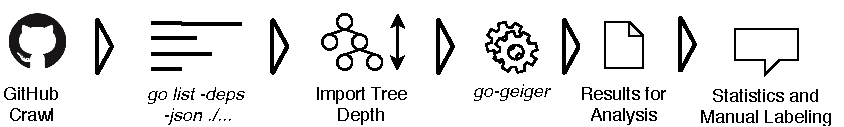
\includegraphics[width=\textwidth]{assets/figures/chapter1/outline.pdf}
    \caption{Thesis Outline and Chapter Relations}
    \label{fig:outline}
\end{figure}

